\documentclass[a4paper,conference,10pt]{IEEEtran}

\usepackage{amsmath,amssymb}
\usepackage{booktabs}
\usepackage{graphicx}
\usepackage{microtype}
\usepackage{url}
\usepackage{xcolor}
\usepackage{balance}

\graphicspath{{../figures/generated/}}
\definecolor{signatureblue}{HTML}{195AA6}
\definecolor{signaturered}{HTML}{BE1E2D}

\title{Subject-Independent Smartphone Activity Recognition\\
with Regularized Generalized Likelihood Ratios}

\author{\IEEEauthorblockN{Shaikh Haris Jamal, Snehil Sanjog, Deepak Pandey, and Jay Daulatkar}
\IEEEauthorblockA{SDET Project\\
International Institute of Information Technology, Hyderabad\\
shaikh.jamal@research.iiit.ac.in\\
\{snehil.sanjog, deepak.pandey, jay.daulatkar\}@students.iiit.ac.in}}

\begin{document}
\maketitle

\begin{abstract}
This work studies whether a compact, interpretable generalized likelihood-ratio test (GLRT) can distinguish six human activities from smartphone accelerometer windows. The classifier fits one regularized multivariate density per activity and assigns a window to the class with the largest fitted likelihood. Its winning-to-runner-up likelihood ratio also supplies a confidence margin. We evaluate the method with subject-independent partitions of UCI HAR and WISDM, so no person appears in both training and test data. A single variance statistic, which was adequate for motion versus stillness, fails to represent the six-class problem. A 15-feature Gaussian GLRT reaches 87.9\% accuracy on UCI HAR and 78.8\% on WISDM. Heavy-tailed Student-$t$ likelihoods provide only small gains. Gravity-aligned motion features combined with regularized discriminant analysis raise WISDM accuracy to 82.6\%, but reduce UCI HAR accuracy by 0.2 percentage points. We therefore retain different training-selected configurations for the two datasets. The confusion structure shows that the remaining problem is not generic motion detection: it is separating similar postures and stair directions under subject and phone-orientation variation.
\end{abstract}

\begin{IEEEkeywords}
human activity recognition, generalized likelihood-ratio test, accelerometer, regularized discriminant analysis, subject-independent evaluation
\end{IEEEkeywords}

\section{Introduction}
Smartphone activity recognition is often presented as a generic classification problem. That description hides two distinct questions. Detecting whether a person is moving can be done with a scalar such as acceleration variance. Distinguishing walking, jogging, stair direction, sitting, standing, and laying requires the joint structure of posture, motion intensity, periodicity, and orientation. A detector designed for the first question can score well while answering the second poorly.

We develop the classifier from the likelihood model upward. Each sensor window is summarized by a small feature vector. Each activity defines a composite hypothesis whose mean and covariance are estimated from training subjects. Classification selects the hypothesis with the greatest fitted likelihood. The likelihood ratio between the best two hypotheses quantifies how strongly the chosen label is preferred. This construction remains a GLRT because the nuisance parameters of every hypothesis are fitted rather than known in advance \cite{kay}.

We test four concrete claims under subject-independent evaluation: whether one variance statistic can support six classes, whether a multivariate Gaussian model is sufficient, whether heavy tails help, and whether gravity-aligned features reduce orientation variability. A candidate is retained only when its training-selected improvement transfers to held-out subjects. That rule leads to different final representations for the two datasets.

The complete implementation, experiment scripts, saved predictions, and figure-generation code are available at \url{https://github.com/Harizz076/smartphone-har-activity-change-detection}.

\section{Background and Related Work}
UCI HAR contains waist-mounted smartphone inertial recordings from 30 volunteers performing six activities \cite{anguita,uci}. Its published processing separates body and gravity acceleration and uses time- and frequency-domain summaries. WISDM contains phone accelerometer recordings from 36 participants in less controlled conditions, with six labels including jogging and stair use \cite{kwapisz}. These datasets serve different purposes here. UCI HAR tests a fixed-placement setting with a standard subject split. WISDM tests greater person and phone-placement variation.

A likelihood-ratio test compares how well competing hypotheses explain an observation. When parameters are unknown, the GLRT substitutes their maximum-likelihood estimates \cite{kay}. With more than two activities, the same principle yields one fitted score per class. The winning score gives the label; the ratio between the first and second scores gives a local measure of ambiguity.

Full class-specific covariance matrices can be noisy. Friedman's regularized discriminant analysis (RDA) interpolates between class-specific, pooled, and spherical covariance estimates using two parameters selected by cross-validation \cite{friedman}. A multivariate Student-$t$ density is a useful rival when Gaussian tails are too light \cite{liurubin}. Orientation-independent HAR methods additionally motivate decomposing acceleration into components parallel and perpendicular to gravity \cite{guo}. These ideas are tested separately so that a gain can be traced to its source.

Online change detection is related but not identical to window classification. Sequential GLRT methods accumulate evidence across time and can combine evidence from several channels \cite{xie,chen}. The packaged UCI HAR data contain shuffled, presegmented windows. WISDM contains activity runs, but gaps and sparse transitions do not support a broad event-timing benchmark. We therefore report six-class window recognition and do not claim a continuous detection score from an artificial stream.

\section{Methodology}
\subsection{Window representation}
For an acceleration window $A=[a_1,\ldots,a_n]$, $a_i\in\mathbb{R}^3$, the original representation contains 15 features: axis means, log variances, pairwise correlations, log jerk energies, dominant frequency, spectral entropy, and log band power. The logarithm compresses positive energy statistics whose raw distributions are strongly right-skewed. This reduces the influence of a few unusually energetic windows and makes a symmetric density a more credible approximation.

The WISDM candidate appends nine orientation-aware features. Let
\begin{equation}
    \hat g=\frac{\bar a}{\lVert\bar a\rVert_2},\qquad
    v_i=a_i^\top\hat g,\qquad
    h_i=\lVert a_i-v_i\hat g\rVert_2 .
\end{equation}
Here $v_i$ is acceleration along the estimated gravity direction and $h_i$ is horizontal magnitude. Their power, jerk, and spectral summaries describe motion in a window-specific frame. The original axis features are retained because their means carry posture information when placement is controlled.

\begin{figure*}[t]
    \centering
    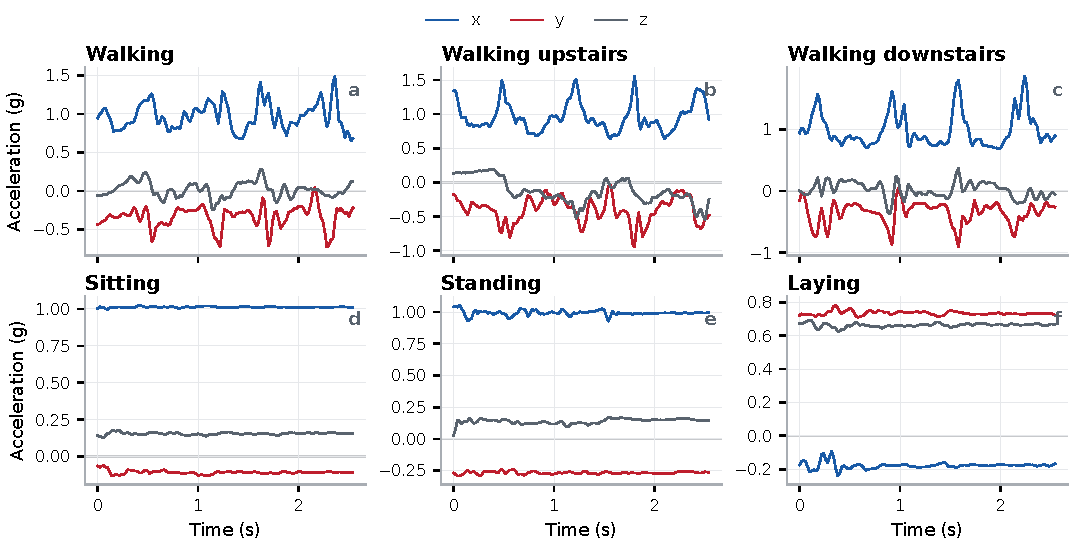
\includegraphics[width=\textwidth]{raw_signal_examples.pdf}
    \caption{Representative held-out UCI HAR windows. Dynamic classes show periodic, multi-axis structure; static classes differ mainly in the gravity projection. A scalar energy statistic discards both patterns. Each window spans 2.56~s at 50~Hz.}
    \label{fig:raw}
\end{figure*}

\subsection{Six-class Gaussian GLRT}
After feature-wise standardization using training data, let $x\in\mathbb{R}^p$ be a test vector. For activity $k$, the hypothesis is
\begin{equation}
    \mathcal H_k:x\sim\mathcal N(\mu_k,\Sigma_k),\quad k=1,\ldots,6.
\end{equation}
The fitted log-likelihood, omitting constants shared by all classes, is
\begin{equation}
 \ell_k(x)=-\frac{1}{2}\left[
 \log|\widehat\Sigma_k|+
 (x-\widehat\mu_k)^\top\widehat\Sigma_k^{-1}(x-\widehat\mu_k)
 \right].
 \label{eq:likelihood}
\end{equation}
Equal class priors are used. Thus $\hat y=\arg\max_k\ell_k(x)$. If $k_1$ and $k_2$ are the first- and second-ranked classes, the reported margin is
\begin{equation}
 G(x)=2\log\frac{\max_{\theta_{k_1}}p(x\mid\mathcal H_{k_1},\theta_{k_1})}
 {\max_{\theta_{k_2}}p(x\mid\mathcal H_{k_2},\theta_{k_2})}
 =2[\ell_{k_1}(x)-\ell_{k_2}(x)].
 \label{eq:glr}
\end{equation}
The factor two is conventional and preserves the decision ordering. A threshold on $G$ can reject uncertain windows, but no rejection threshold is tuned for the primary results.

\subsection{Covariance regularization and heavy-tailed rival}
For class scatter $S_k$, pooled within-class scatter $S$, class weight $W_k$, and total weight $W$, RDA first mixes class and pooled estimates:
\begin{align}
 S_k(\lambda)&=(1-\lambda)S_k+\lambda S,\\
 W_k(\lambda)&=(1-\lambda)W_k+\lambda W,\\
 \widetilde\Sigma_k(\lambda)&=S_k(\lambda)/W_k(\lambda).
\end{align}
It then shrinks the eigenvalues toward their mean:
\begin{equation}
 \widehat\Sigma_k=(1-\gamma)\widetilde\Sigma_k+
 \gamma\frac{\operatorname{tr}(\widetilde\Sigma_k)}{p}I+10^{-6}I.
 \label{eq:rda}
\end{equation}
$\lambda=0$ preserves class-specific geometry; $\lambda=1$ uses a pooled covariance. $\gamma=1$ produces a spherical estimate. Both are chosen using training subjects only. We also replace the Gaussian density with a multivariate Student-$t$ density as a heavy-tailed sensitivity analysis. Its degrees of freedom and covariance regularization are selected by the same training-fold protocol.

\section{Experimental Setup}
Table~\ref{tab:data} summarizes the evaluation. UCI HAR uses its published subject-independent partition. WISDM subjects are divided once into 24 training and 12 test participants; the test identities remain fixed across models. Its raw stream is split within each uninterrupted subject-activity run into non-overlapping 200-sample windows, corresponding to 10~s at 20~Hz. Incomplete tails are discarded. No window from a test subject is used for standardization, feature selection, covariance fitting, or hyperparameter selection.

\begin{table}[t]
\caption{Subject-independent datasets and windows}
\label{tab:data}
\centering
\begin{tabular}{lrrrcc}
\toprule
Dataset & Hz & Length & Features & Train & Test \\
\midrule
UCI HAR & 50 & 128 & 15 & 7,352 & 2,947 \\
WISDM & 20 & 200 & 24 & 3,597 & 1,628 \\
\bottomrule
\end{tabular}
\vspace{2pt}
\footnotesize UCI uses 21 training and 9 test subjects; WISDM uses 24 and 12.
\end{table}

Model selection maximizes balanced accuracy over subject-disjoint training folds. This objective prevents common activities from determining every choice. Final reporting includes ordinary accuracy, balanced accuracy, macro F1, per-class recall, and the confusion matrix. Values are rounded to one decimal percentage point because finer precision is not operationally meaningful for these fixed cohorts.

The variance baseline uses the earlier scalar motion statistic. The Gaussian GLRT uses the 15-feature representation. The Student-$t$ row changes only the density. The final UCI configuration uses the 15 features with $(\lambda,\gamma)=(0,0.03)$. The final WISDM configuration uses all 24 features with $(0.25,0.01)$. Every table and plot is generated from saved predictions by repository code. The analysis and figure audit follow a documented scientific workflow \cite{kassis}.

\section{Results and Analysis}
\subsection{From motion detection to six activities}
Figure~\ref{fig:performance} gives the central comparison. The scalar baseline reaches 37.9\% accuracy on UCI HAR and 58.1\% on WISDM. Its higher WISDM value reflects the separability of jogging and static behavior, not reliable six-class recognition. The multivariate Gaussian model adds roughly 50 points on UCI HAR and 21 points on WISDM because it retains posture, periodicity, and cross-axis dependence.

\begin{figure*}[t]
    \centering
    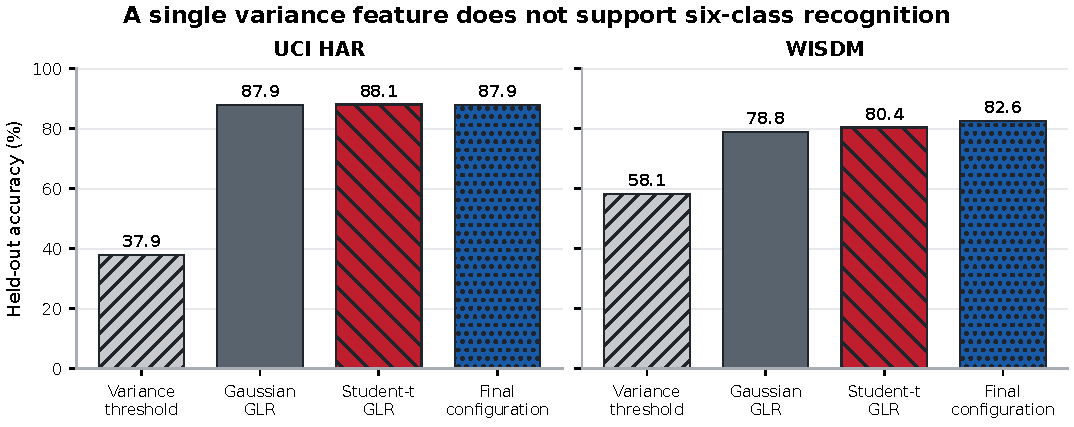
\includegraphics[width=0.94\textwidth]{performance_overview.pdf}
    \caption{Held-out six-class accuracy. The heavy-tailed density gives a small change; feature geometry and subject variation matter more. The final configuration is selected separately for each dataset using training subjects.}
    \label{fig:performance}
\end{figure*}

Student-$t$ likelihoods change UCI HAR accuracy from 87.9\% to 88.1\% and WISDM from 78.8\% to 80.4\%. This is evidence that outliers contribute to WISDM error, but it does not explain most failures. The larger WISDM gain comes from gravity-aligned features with RDA, which reach 82.6\% accuracy and 80.7\% balanced accuracy. The same 24-feature candidate scores 87.7\% on UCI HAR, 0.2 points below the original representation. Its cross-validation gain did not transfer, so it is not used as the UCI final model.

\begin{table}[t]
\caption{Held-out performance, percent}
\label{tab:results}
\centering
\begin{tabular}{llrrr}
\toprule
Dataset & Model & Acc. & Bal. acc. & Macro F1 \\
\midrule
UCI & Variance & 37.9 & -- & -- \\
UCI & Gaussian GLRT & 87.9 & 87.8 & 87.7 \\
UCI & Student-$t$ GLRT & 88.1 & 87.9 & 87.8 \\
UCI & Final & 87.9 & 87.8 & 87.7 \\
\midrule
WISDM & Variance & 58.1 & -- & -- \\
WISDM & Gaussian GLRT & 78.8 & 78.4 & 76.7 \\
WISDM & Student-$t$ GLRT & 80.4 & 79.7 & 78.0 \\
WISDM & Final & 82.6 & 80.7 & 78.1 \\
\bottomrule
\end{tabular}
\end{table}

\subsection{What the errors mean}
Figure~\ref{fig:confusion} separates two failure modes. In UCI HAR, 36\% of sitting windows are called standing, whereas laying is identified without error. The dynamic classes exceed 86\% recall. The phone's stable waist orientation therefore carries enough information for broad posture and motion separation, but sitting and standing occupy overlapping feature regions for some participants.

WISDM has a different bottleneck. Jogging recall is 95.7\%, yet upstairs recall is 47.0\%. Of the upstairs windows, 39\% are called downstairs and 14\% jogging. Walking also leaks into downstairs. These are directional and placement-sensitive errors. Gravity alignment improves the overall geometry but horizontal magnitude removes directional cues that could distinguish ascent from descent. Retaining the original axes limits this loss but does not remove it.

\begin{figure*}[t]
    \centering
    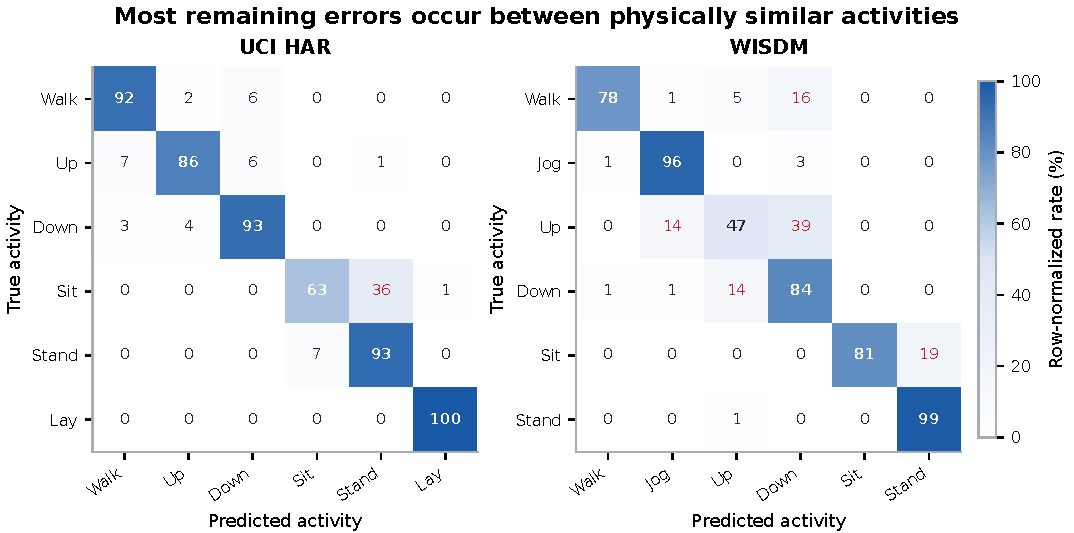
\includegraphics[width=0.93\textwidth]{confusion_matrices.pdf}
    \caption{Row-normalized confusion matrices for the final configurations. Numbers are percentages within each true class. Static posture is the UCI bottleneck; stair direction is the WISDM bottleneck.}
    \label{fig:confusion}
\end{figure*}

\begin{table}[t]
\caption{Final per-class recall, percent}
\label{tab:recall}
\centering
\begin{tabular}{lrlr}
\toprule
UCI class & Recall & WISDM class & Recall \\
\midrule
Walking & 91.9 & Walking & 78.2 \\
Upstairs & 86.2 & Jogging & 95.7 \\
Downstairs & 92.9 & Upstairs & 47.0 \\
Sitting & 62.5 & Downstairs & 83.6 \\
Standing & 93.0 & Sitting & 81.1 \\
Laying & 100 & Standing & 98.9 \\
\bottomrule
\end{tabular}
\end{table}

\subsection{Average gain versus subject variation}
The WISDM improvement is not uniform. Figure~\ref{fig:subjects} shows paired results for the 12 test subjects. Several subjects gain substantially, while others change little or regress. One participant remains near 35\% accuracy under both models. This spread is larger than the 3.8-point average gain and prevents a claim that gravity alignment solves cross-person generalization.

\begin{figure}[t]
    \centering
    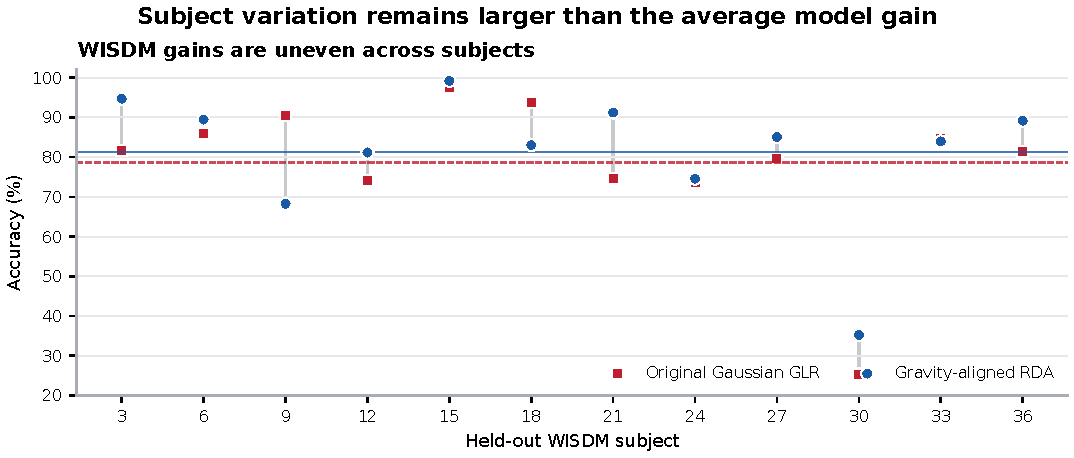
\includegraphics[width=\columnwidth]{subject_variation.pdf}
    \caption{WISDM accuracy by held-out subject. Lines connect the same participant under the original Gaussian GLRT and the gravity-aligned RDA model. Horizontal lines show their subject means.}
    \label{fig:subjects}
\end{figure}

The GLR margin remains useful even without a tuned threshold. Retaining only the half of UCI HAR windows with the largest margins yields 98.0\% accuracy; the analogous WISDM subset reaches 96.0\%. At full coverage the values return to the primary accuracies. This ordering suggests a practical reject option for applications that can defer uncertain decisions. It does not calibrate $G$ as a probability, and the rejection threshold would need an independent validation set.

\section{Discussion and Inferences}
Three inferences follow from the experiments. First, the mathematical form of a GLRT does not make an impoverished observation informative. The variance baseline asks a motion-intensity question, so poor six-class performance is expected even though the detector itself is valid. The improvement comes from defining hypotheses over features that express the differences of interest.

Second, distributional flexibility has diminishing returns when representation error dominates. Student-$t$ tails help WISDM slightly. Full covariance pooling on the original features is rejected by training folds, which select $\lambda=0$. In contrast, changing the coordinate system with gravity-aligned features gives a larger gain. This points to nuisance orientation and subject behavior, rather than Gaussianity alone, as the more consequential mismatch.

Third, model selection must be allowed to produce different answers. The gravity candidate improves WISDM but not UCI HAR. Adopting it everywhere would turn a local success into a small UCI regression. The final system therefore shares the likelihood-ratio framework while permitting dataset-specific feature and covariance choices.

The study has four limitations. The held-out sets were inspected during earlier development, so the final results are exploratory rather than confirmatory. WISDM windows are long and non-overlapping; short activities and transition timing are outside the evaluation. Accelerometer-only features cannot recover all contextual differences between stair directions. Finally, a fixed subject split gives limited evidence about uncertainty across possible cohorts. A repeated subject-level evaluation or a new external cohort would support stronger generalization claims.

\section{Conclusion and Future Work}
A six-class GLRT can be both interpretable and competitive when its hypotheses are built on informative, regularized feature distributions. The final models achieve 87.9\% accuracy on UCI HAR and 82.6\% on WISDM under subject-independent testing. The error structure matters more than the aggregate score: UCI HAR is limited by sitting versus standing, while WISDM is limited by stair direction and one difficult participant.

The next experiment should collect or adopt a dataset with continuous timestamps, diverse transitions, and event annotations. A sequential detector can then accumulate per-sample or short-block likelihood evidence, reset after decisions, and measure detection delay against false alarms. For six-class recognition, gyroscope features and a direction-preserving body frame are stronger candidates than simply adding more scalar summaries. Confidence calibration on unseen subjects would also turn the GLR margin into a defensible reject rule.

\balance
\begin{thebibliography}{12}

\bibitem{kay}
S. M. Kay, \emph{Fundamentals of Statistical Signal Processing, Volume II: Detection Theory}. Upper Saddle River, NJ, USA: Prentice Hall, 1998.

\bibitem{anguita}
D. Anguita, A. Ghio, L. Oneto, X. Parra, and J. L. Reyes-Ortiz, ``A public domain dataset for human activity recognition using smartphones,'' in \emph{Proc. ESANN}, 2013, pp. 437--442.

\bibitem{uci}
J. L. Reyes-Ortiz, D. Anguita, A. Ghio, L. Oneto, and X. Parra, ``Human Activity Recognition Using Smartphones,'' UCI Machine Learning Repository, 2012, doi: 10.24432/C54S4K.

\bibitem{kwapisz}
J. R. Kwapisz, G. M. Weiss, and S. A. Moore, ``Activity recognition using cell phone accelerometers,'' \emph{SIGKDD Explor.}, vol. 12, no. 2, pp. 74--82, 2011, doi: 10.1145/1964897.1964918.

\bibitem{friedman}
J. H. Friedman, ``Regularized discriminant analysis,'' \emph{J. Amer. Stat. Assoc.}, vol. 84, no. 405, pp. 165--175, 1989, doi: 10.1080/01621459.1989.10478752.

\bibitem{liurubin}
C. Liu and D. B. Rubin, ``ML estimation of the $t$ distribution using EM and its extensions, ECM and ECME,'' \emph{Statistica Sinica}, vol. 5, no. 1, pp. 19--39, 1995.

\bibitem{guo}
H. Guo, L. Chen, G. Chen, and M. Lv, ``Smartphone-based activity recognition independent of device orientation and placement,'' \emph{Int. J. Commun. Syst.}, vol. 29, no. 16, pp. 2403--2415, 2016, doi: 10.1002/dac.3010.

\bibitem{xie}
Y. Xie and D. Siegmund, ``Sequential multi-sensor change-point detection,'' \emph{Ann. Statist.}, vol. 41, no. 2, pp. 670--692, 2013, doi: 10.1214/13-AOS1094.

\bibitem{chen}
Y. Chen, T. Wang, and R. J. Samworth, ``High-dimensional, multiscale online changepoint detection,'' \emph{J. R. Stat. Soc. B}, vol. 84, no. 1, pp. 234--266, 2022.

\bibitem{kassis}
T. Kassis, V. Agarwal, Y. He, D. Patel, and A. M. Brueckner, ``Scientific Agent Skills: A library of procedural knowledge for research agents,'' arXiv:2609.00065, 2026, doi: 10.48550/arXiv.2609.00065.

\end{thebibliography}

\end{document}
